\chapterold{Fibonacci numbers}

Another widespread example used in programming textbooks is a recursive function 
that generates the Fibonacci numbers\footnote{\url{http://go.yurichev.com/17332}}.
The sequence is very simple: each consecutive number is the sum of the previous two.
The first two numbers are 1's or 0, 1 and 1.

The sequence starts like this:

\begin{center}
$0, 1, 1, 2, 3, 5, 8, 13, 21, 34, 55, 89, 144, 233, 377, 610, 987, 1597, 2584, 4181 ...$
\end{center}

\sectionold{Example \#1}

The implementation is simple. This program generates the sequence until 21.

\lstinputlisting{\CURPATH/fib.c}

\lstinputlisting[caption=MSVC 2010 x86]{\CURPATH/fib.asm}

We will illustrate the stack frames with this.

\clearpage

Let's load the example in \olly and trace to the last call of \ttf{}:

\begin{figure}[H]
\centering
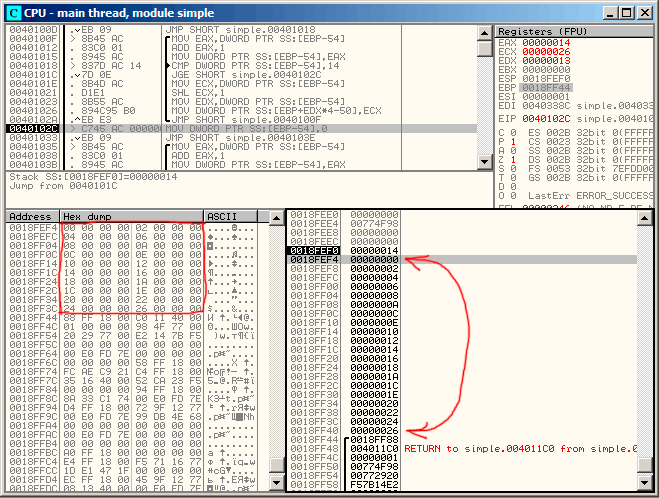
\includegraphics[scale=\FigScale]{\CURPATH/olly.png}
\caption{\olly: last call of \ttf{}}
\label{fig:fib_olly}
\end{figure}

\clearpage
Let's investigate the stack more closely. 
Comments were added by the author of this book
\footnote{By the way, it's possible to select several entries in \olly and copy them to the clipboard (Ctrl-C).
That's what was done for this example.}:

\lstinputlisting{\CURPATH/stack_EN.txt}

The function is recursive \footnote{i.e., it calls itself}, hence stack looks like a \q{sandwich}.

We see that the \IT{limit} argument is always the same (\TT{0x14} or 20), but the $a$ and $b$ arguments are different for each call.

There are also the \ac{RA}-s and the saved \EBP values.
\olly is able to determine the EBP-based frames, so it draws these brackets.
The values inside each bracket make the \gls{stack frame}, 
in other words, the stack area which each function incarnation uses as scratch space. 

We can also say that each function incarnation must not access
stack elements beyond the boundaries of its frame (excluding function arguments), 
although it's technically possible. 

It's usually true, unless the function has bugs.

Each saved \EBP value is the address of the previous \gls{stack frame}: 
this is the reason why some debuggers can easily divide the stack in frames and dump each 
function's arguments.
% TODO add about StackWalk (MSDN)

As we see here, each function incarnation prepares the arguments for the next function call.

At the end we see the 3 arguments for \main. 
\TT{argc} is 1 (yes, indeed, we have ran the program without command-line arguments).

This easily to lead to a stack overflow: just remove (or comment out) the limit check and it will crash with
exception \TT{0xC00000FD} (stack overflow.)

\sectionold{Example \#2}

My function has some redundancy, so let's add a new local variable \IT{next} and replace all \q{a+b} with it:

\lstinputlisting{\CURPATH/fib2.c}

This is the output of non-optimizing MSVC, so the \IT{next} variable is actually allocated 
in the local stack:

\lstinputlisting[caption=MSVC 2010 x86]{\CURPATH/fib2.asm}

\clearpage
Let's load it in \olly once again:

\begin{figure}[H]
\centering
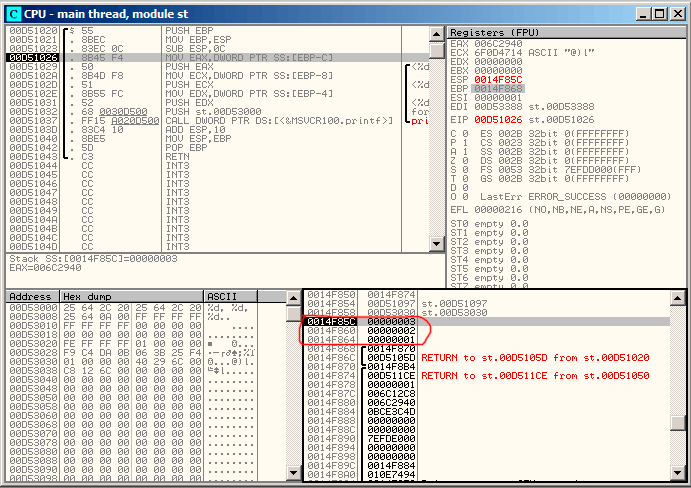
\includegraphics[scale=\FigScale]{\CURPATH/olly2.png}
\caption{\olly: last call of \ttf{}}
\label{fig:fib_olly2}
\end{figure}

Now the \IT{next} variable is present in each frame.

\clearpage

Let's investigate the stack more closely. The author has again added his comments:

\lstinputlisting{\CURPATH/stack2_EN.txt}

% FIXME what a word! hmmm...
Here we see it: the \IT{next} value is calculated in each function incarnation, then passed as
argument $b$ to the next incarnation.

\sectionold{Summary}

\label{Recursion_and_tail_call}
\myindex{\Recursion}
Recursive functions are \ae{}sthetically nice, but technically may degrade performance because
of their heavy stack usage.
Everyone who writes performance critical code probably should should avoid recursion.

For example, the author of this book once wrote a function to seek a particular node in a binary tree. 
As a recursive function it looked quite stylish but since additional time
was spent at each function call
for the prologue/epilogue, it was working a couple of times slower than an iterative (recursion-free)
implementation.

\newcommand{\FnFP}{\footnote{LISP, Python, Lua, \etc{}.}}
\myindex{\Recursion!Tail recursion}

By the way, that is the reason that some functional \ac{PL}\FnFP{} compilers (where recursion is used heavily) use \gls{tail call}.
